\documentclass{extbook}[14pt]
\usepackage{multicol, enumerate, enumitem, hyperref, color, soul, setspace, parskip, fancyhdr, amssymb, amsthm, amsmath, bbm, latexsym, units, mathtools}
\everymath{\displaystyle}
\usepackage[headsep=0.5cm,headheight=0cm, left=1 in,right= 1 in,top= 1 in,bottom= 1 in]{geometry}
\pagestyle{fancy}
\lhead{}
\chead{Answer Key for Module\,12L\,-\,Graphing\,Rational\,Functions Version C}
\rhead{}
\lfoot{Summer\,C\,2020}
\cfoot{}
\rfoot{}
\begin{document}
\textbf{This key should allow you to understand why you choose the option you did (beyond just getting a question right or wrong). \href{https://xronos.clas.ufl.edu/mac1105spring2020/courseDescriptionAndMisc/Exams/LearningFromResults}{More instructions on how to use this key can be found here}.}

\textbf{If you have a suggestion to make the keys better, \href{https://forms.gle/CZkbZmPbC9XALEE88}{please fill out the short survey here}.}

\textit{Note: This key is auto-generated and may contain issues and/or errors. The keys are reviewed after each exam to ensure grading is done accurately. If there are issues (like duplicate options), they are noted in the offline gradebook. The keys are a work-in-progress to give students as many resources to improve as possible.}

\rule{\textwidth}{0.4pt}

76. Determine the vertical asymptotes and holes in the rational function below.
\[ f(x) = \frac{16x^{3} -48 x^{2} -25 x + 75}{16x^{2} -32 x + 15} \] 
The solution is $ \text{Vertical Asymptote of } x = 0.75 \text{ and hole at } x = 1.25 $ 

\begin{enumerate}[label=\Alph*.] 
\item $ \text{Vertical Asymptotes of } x = 0.75 \text{ and } x = 1.25 \text{ with no holes.} $ 

 This corresponds to not factoring out the hole. 
\item $ \text{Holes at } x = 0.75 \text{ and } x = 1.25 \text{ with no vertical asymptotes.} $ 

 This corresponds to considering where the denominator is equal to 0 as holes. 
\item $ \text{Vertical Asymptotes of } x = 0.75 \text{ and } x = -1.25 \text{ with a hole at } x = 1.25 $ 

 This corresponds to setting the numerator equal to 0. 
\item $ \text{Vertical Asymptote of } x = 1.0 \text{ and hole at } x = 1.25 $ 

 This corresponds to mixing vertical and horizontal asymptotes. 
\item $ \text{Vertical Asymptote of } x = 0.75 \text{ and hole at } x = 1.25 $ 

 This is the correct answer. 
\end{enumerate} 
 
General Comments: Remember to factor the numerator and denominator. Any factors that cancel are holes in the function. The zeros left in the denominator are the vertical asymptotes.

-----------------------------------------------

77. Which of the following functions \textit{could} be the graph below?
\begin{center} 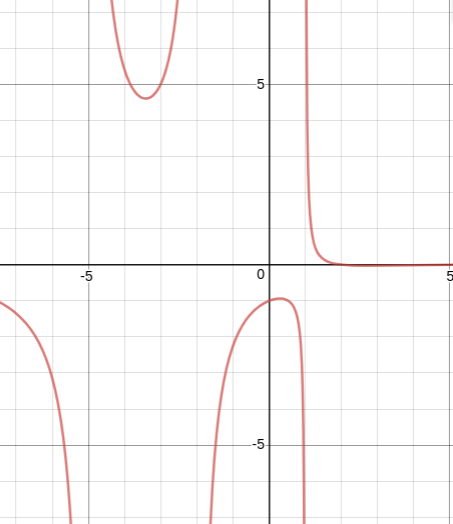
\includegraphics[width=0.3\textwidth]{../Figures/identifyGraphOfRationalFunctionC.png} \end{center} 

The solution is $ f(x) = \frac{x^{3} +4 x^{2} -15 x -18}{x^{3} +6 x^{2} +3 x -10} $ 

\begin{enumerate}[label=\Alph*.] 
\item $ f(x) = \frac{x^{3} +4 x^{2} -17 x -60}{x^{3} +5 x^{2} +2 x -8} $ 

 This function has vertical asymptotes at $x=-2$, and $x=1$. 
\item $ f(x) = \frac{x^{3} +7 x^{2} +7 x -15}{x^{3} -6 x^{2} +3 x + 10} $ 

 This function has vertical asymptotes at $x=-1$, $x=2$, and $x=5$. 
\item $ f(x) = \frac{x^{3} + x^{2} -26 x + 24}{x^{3} +3 x^{2} -6 x -8} $ 

 This function has vertical asymptotes at $x=-1$, and $x=2$. 
\item $ f(x) = \frac{x^{3} +4 x^{2} -15 x -18}{x^{3} +6 x^{2} +3 x -10} $ 

 This function has vertical asymptotes at $x=-5$, $x=-2$, and $x=1$. 
\item $ \text{None of the above are possible equations for the graph.} $ 

 If you believe none of the functions above could be the graph, please contact the coordinator. 
\end{enumerate} 
 
\textbf{General comments:} To determine whether the function could be the graph, determine the vertical asymptotes of the graph.

-----------------------------------------------

78. Determine the horizontal and/or oblique asymptotes in the rational function below.
\[ f(x) = \frac{8x^{3} -28 x^{2} -10 x + 12}{8x^{3} +22 x^{2} -x -15} \] 
The solution is $ \text{Horizontal Asymptote of } y = 1.000  $ 

\begin{enumerate}[label=\Alph*.] 
\item $ \text{None of the above} $ 

 This corresponds to believing there should be an oblique asymptote. 
\item $ \text{Horizontal Asymptote of } y = 0  $ 

 This corresponds to using the rule for Horizontal Asymptote when the degree of the denominator is larger than the numerator. 
\item $ \text{Vertical Asymptote of } y = 2.000  $ 

 This corresponds to the hole at $x = 2.000$. 
\item $ \text{Vertical Asymptote of } y = -1  $ 

 This corresponds to the hole at $x = -1$. 
\item $ \text{Horizontal Asymptote of } y = 1.000  $ 

 * This is the correct option. 
\end{enumerate} 
 
General Comments: We have a Horizontal Asymptote if the degree of the numerator is smaller than or equal to the degree of the denominator. We have an Oblique Asymptote if the degree of the numerator is larger than the degree of the denominator. We cannot have both!

-----------------------------------------------

79. Determine the horizontal and/or oblique asymptotes in the rational function below.
\[ f(x) = \frac{12x^{3} -19 x^{2} -3 x + 10}{4x^{2} -13 x + 10} \] 
The solution is $ y = 3x + 5 $ 

\begin{enumerate}[label=\Alph*.] 
\item $ \text{Horizontal Asymptote of } y = 3.0 \text{ and Oblique Asymptote of } y = 3x + 5 $ 

 This corresponds to believing there can be both a horizontal and oblique asymptote. 
\item $ \text{Oblique Asymptote of } y = 3x + 5. $ 

 This is the correct answer. 
\item $ \text{Horizontal Asymptote at } y = 2.0 $ 

 This corresponds to considering where the denominator is equal to 0 as horizontal asymptote. 
\item $ \text{Horizontal Asymptote of } y = 2.0 \text{ and Oblique Asymptote of } y = 3x + 5 $ 

 This corresponds to believing there can be both a horizontal and oblique asymptote AND mixing up horizontal/vertical asymoptote. 
\item $ \text{Horizontal Asymptote of } y = 3.0  $ 

 This corresponds to using rule for Horizontal Asymptote when degree of numerator and denominator match. 
\end{enumerate} 
 
General Comments: We have a Horizontal Asymptote if the degree of the numerator is smaller than or equal to the degree of the denominator. We have an Oblique Asymptote if the degree of the numerator is larger than the degree of the denominator. We cannot have both!

-----------------------------------------------

80. Determine the vertical asymptotes and holes in the rational function below.
\[ f(x) = \frac{6x^{3} + x^{2} -30 x -25}{6x^{2} +x -15} \] 
The solution is $ \text{Vertical Asymptote of } x = 1.5 \text{ and hole at } x = -1.667 $ 

\begin{enumerate}[label=\Alph*.] 
\item $ \text{Vertical Asymptote of } x = 1.5 \text{ and hole at } x = -1.667 $ 

 This is the correct answer. 
\item $ \text{Vertical Asymptotes of } x = 1.5 \text{ and } x = 2.5 \text{ with a hole at } x = -1.667 $ 

 This corresponds to setting the numerator equal to 0. 
\item $ \text{Holes at } x = 1.5 \text{ and } x = -1.667 \text{ with no vertical asymptotes.} $ 

 This corresponds to considering where the denominator is equal to 0 as holes. 
\item $ \text{Vertical Asymptote of } x = 1.0 \text{ and hole at } x = -1.667 $ 

 This corresponds to mixing vertical and horizontal asymptotes. 
\item $ \text{Vertical Asymptotes of } x = 1.5 \text{ and } x = -1.667 \text{ with no holes.} $ 

 This corresponds to not factoring out the hole. 
\end{enumerate} 
 
General Comments: Remember to factor the numerator and denominator. Any factors that cancel are holes in the function. The zeros left in the denominator are the vertical asymptotes.

-----------------------------------------------


\end{document}

